Existem diversos \textit{benchmarks} que especificam e simulam cargas de trabalho para avaliarem sistemas computacionais. No entanto, não existe nenhum \textit{benchmark} estimule a sua dinâmica e que possibilite uma avaliação em regime transiente. Este capítulo apresenta e defini uma metodologia de extensão de avaliação em regime transiente para \textit{benchmarks} aproveitando toda a sua maturidade e robustez.

\section{Estratégicas de extensão}

O \textit{benchmark} bench4Q define uma carga de trabalho, incluindo banco de dados, transações, regras de execução e de taxa de transferência e métricas de resposta.  Para expor a dinâmica de um sistema é necessário estimulá-lo, a carga de trabalho é quem estimulará o sistema através de cenários ou fenômenos de \textit{burstiness}. Essa implementação é composta por classes ou funções, influenciado diretamente pela linguagem em que o \textit{benchmark} foi desenvolvido, esse conjunto de código é um componente básico do \textit{benchmark} que refere-se a uma unidade de trabalho genérico que envia a carga para o sistema. Alguns \textit{benchmarks} incluem solicitações HTTP, chamadas de procedimento remoto, invocações de serviços Web, transações de banco de dados, comandos interativos ou também mesmo poderia ser composto de múltiplas tarefas de processamento, por exemplo sessões de cliente que compreendem várias solicitações ao sistema, etc \cite{Kounev2005}. Segundo \cite{Nobile2013} uma alteração na entrada (carga de trabalho) fará com que o sistema saia do estado de regime estacionário e entre em um período de regime transiente e para descrever a dinâmica de um sistema, comumente, o ganho em regime estacionário é calculado para uma entrada degrau unitário.

O objetivo deste trabalho é estender a carga de trabalho do \textit{benchmark} de tal maneira que permite-se estimular o sistemas a apresentar a sua dinâmica, assim possibilitando a analise transiente do sistema. 

%Devemos ter em conta que dentro da nuvem existem recursos com maior escalabilidade

%Além disso, nós quantificar a sobrecarga de desempenho para HA em comparação com o sistema de não-HA durante as operações normais. Temos utilizado este método para impulsionar melhorias na disponibilidade SQL Server. Embora a metodologia não é específico para a carga de trabalho TPC-E ou o Microsoft SQL Server, não estamos tentando definir um "uso geral" HA referência neste documento.
\cite{Binnig2009} os serviços em nuvem de hoje diferem entre outros pelo custo, desempenho, garantias de consistência, balanceamento de carga, \textit{caching}, tolerância a falhas, SLA e linguagem de programação. Para a discussão deste trabalho, assumimos um sistema de \textit{n-tiers} que consiste nos seguintes componentes:

\begin{description}
	\item[Gerador de Carga (\textit{Workload}) :]
	\item[Balanceador de carga (\textit{Load Balancer}):]
	\item[Servidor Físico (\textit{Hypervisor}):]
	%O hipervisor, também conhecido como virtualizador, é um componente de software que hospeda as VMs e é responsável pela virtualização e controle dos recursos compartilhados pelas máquinas virtuais, tais como, processadores, dispositivos de entrada e saída e memória (Rose, 2004)	(Carissimi, 2008). Além disso, ele deve escalonar qual máquina virtual executará a cada momento, semelhante ao escalonador de processos do sistema operacional (Menascé, 2005).
	\item[Servidor de dados (\textit{Data base}):]	
\end{description}



%FALAR SOBRE OS TIPOS DE GERENCIAMENTO DE RECURSO, LER O ARTIGO A Survey of Resource Management in Multi-Tier Web Applications.
%De acordo com o grau de disponibilidade e necessidade da aplicação, uma VM pode ser iniciada  precisar de redundância em várias camadas, como fonte de alimentação, armazenamento (por exemplo, níveis de disco RAID), NICs e switches de rede, número de instâncias de banco de dados standby, eo sistema duplicado em dados remoto central (para a recuperação de desastres geográfica). Neste artigo vamos nos concentrar em como o RDBMS lida com várias falhas. 
%Failover se refere à transição do serviço de Principal para Standby Server. Idealmente, o sistema de banco de dados pode failover automaticamente, sem intervenção administrativa para o tempo de inatividade não planejado. O administrador normalmente inicia um processo de failover 'manual' para o tempo de inatividade planejado. Failback refere-se à transferência de serviço de volta para o servidor principal original (após planejado / tempo de inatividade não planejado). A operação é muitas vezes semelhante ao failover manual, exceto que os servidores do Principal / Standby são viradas.

%A Figura 1 mostra os principais componentes no ambiente de teste. Note que a definição System- Sub-Test (SUT) no benchmark TPC-E é estendido para incluir o componente de conectividade, que pode ser executado em ambos fisicamente a máquina Motorista TPC-E (por exemplo, SQL Server Native Client para Database Mirroring) ou uma máquina de servidor (por exemplo, nome de rede virtual para Failover Clustering).
%Para simular o tempo de inatividade planejado, podemos chamar APIs de failover fornecidos pelo RDBMS durante a execução da carga de trabalho TPC-E. Para o tempo de inatividade não planejada, precisamos simular vários eventos perturbadores que possam ocorrer no sistema. A Tabela 1 mostra alguns exemplos de falha.

%Em nosso modelo, assumimos que o sistema segue o princípio de "fail-fast 'descrito por Gray e Siewiorek [4]. Desde que as falhas em hardware e software causar falhas imediatas, não é necessário testar através de um conjunto exaustivo de modos de falha.
%Assim nós não tentar enumerar uma lista "completa" de falhas. O atributo fail-fast devem ser verificadas independentemente do teste de desempenho.


A carga de trabalho Bench4Q é estendida para abranger os seguintes cenários:
\begin{itemize}
	\item a dinâmica do sistema: um período de tempo em que o sistema fica sobrecarregado, acarretando negativamente efeitos colaterais em cascata, e com o decorrer do tempo este efeito seja neutralizado e harmonizado pelo sistema. %• o tempo de inatividade planejado: Um período de tempo de paradas programadas para manutenção do sistema, caracterizado por uma transição ordenada de serviço de Principal para Standby Server. As causas das interrupções programadas incluem patches de OS & SQL, service pack, manutenção de hardware, manutenção on-line, etc.
	\item %• o tempo de inatividade não planejado: Um período de tempo de inatividade não programado, muitas vezes devido a vários falhas, tais como falhas de hardware, erros de software e erros humanos, causando uma transição abrupta do serviço de Principal de espera do servidor.		
\end{itemize}


\subsection{Métricas}
A metodologia de extensão descreve as etapas necessárias para as modificações, a presente metodologia permite que se obtenha uma carga de trabalho que estimule o sistemas a apresentar a sua dinâmica, assim possibilita a analise transiente do sistema. De acordo com \cite{KaiSachs2010}, uma metodologia de desenvolvimento de \textit{benchmarks} deve incluir em seu processo de desenvolvimento, bem como a sua execução e a análise dos seus resultados. Para tanto é necessário medir o comportamento do sistema com a base me métricas. A métrica é uma função que transforma resultados medidos em uma forma facilmente compreendida. \cite{Folkerts2013} As métricas de referência deve permitir caracterizar e quantificar o comportamento do sistema quando enfrenta perturbações (ou seja, falhas, ataques, e variações de ambiente operacional).\cite{Marco2012} As métricas tradicionais, de analise estacionaria, não podem capturar os comportamentos transitórios do sistema em resposta às variações de carga implementada no primeiro passo dessa metodologia.

No contexto de avaliação transiente, \cite{Rosu1997} afirma que a reatividade da métrica é muitas vezes mais importante do que a otimização da mesma, no mesmo trabalho, \cite{Rosu1997} apresenta a característica e comportamento de uma métrica transiente, conforme ilustrado pela figura \ref{fig:transient-metric}, que são: 
\begin{itemize}
	\item \textbf{\textit{Reaction Time} (Tempo de reação)} - o período entre a ocorrência da variação crítica e a conclusão da promulgação realocação de correção;
	
	\item \textbf{\textit{Recovery Time} (Tempo de Recuperação)}  - o intervalo entre a conclusão promulgação e da restauração de um nível de desempenho aceitável;
	
	\item \textbf{\textit{Performance Laxity} (Frouxidão performance)} - a diferença entre o required v performance, e o desempenho em estado estacionário, após a redistribuição;
\end{itemize}


\begin{figure}[!htb]
	\caption{Comportamento de métrica transiente}
	\label{fig:transient-metric}
	\centering
	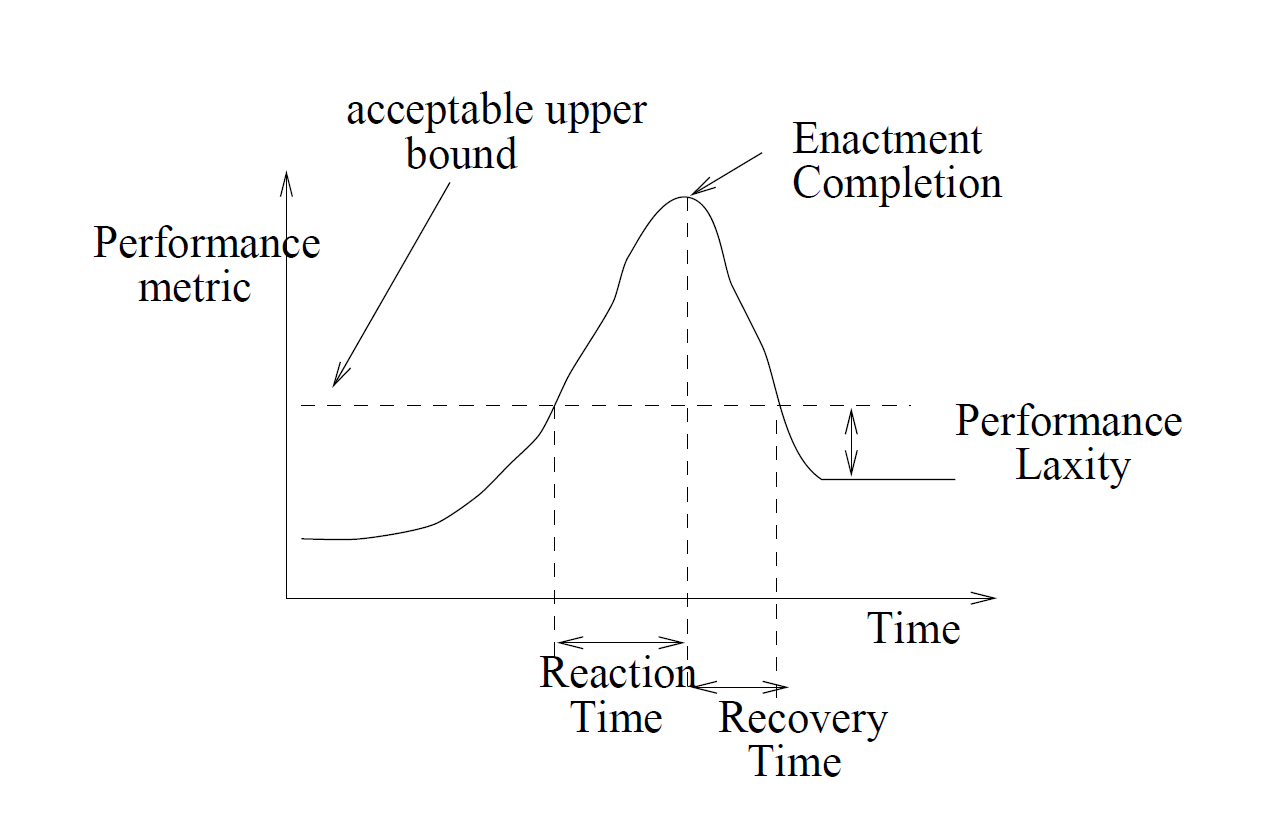
\includegraphics[scale=0.4]{transient-metric.png}
	\fdireta{Rosu1997}		
\end{figure}


A métrica em questão deve ser identifica dentro da realidade e necessidade em que se encontra o sistemas a ser avaliado. Logo será de uma ingenuidade fixar uma métrica para um sistema desconhecido, o importante é que ela tenha o comportamento e as caracteriais apresentadas anteriormente nesse passo da metodologia de extensão. Existem diversos trabalhos dedicados que identificam métricas transiente em vários contextos como o \cite{Binnig2009, Lu2000, Rosu1997}.

\cite{Binnig2009} afirma que os \textit{benchmarks} tradicionais são principalmente preocupados com o desempenho e o custo de sistemas estáticos e essas métricas ainda tem relevância para as aplicações em nuvem, mas é necessário medir diferentes métricas para sistemas escaláveis (ou seja, dinâmico) onde os recursos vêm e vão. Ainda \cite{Binnig2009} enfatiza que os novos \textit{benchmarks} devem relatar métricas diferentes do que os benchmarks existentes: 
\begin{citacao}
Em vez de medir o desempenho médio de um sistema estático em carga máxima, as novas métricas devem refletir a capacidade dos serviços em nuvem para se adaptar a uma mudança de carga com relação ao desempenho e custos. Além disso, uma métrica adicional também deve cobrir a robustez desses serviços contra falhas de nós individuais.
\end{citacao}


%
As métricas definidas precisam refletir o cenários de dinâmica do sistema, que inclui três aspectos principais:
\begin{description}
	\item[Conexões por segundo (Load Balancer):] Conforme sugerido por \cite{Binnig2009}, medir a escalabilidade através do aumento dos interações web emitidos por segundo ao longo do tempo e de forma contínua contando o interação web que são respondidas em um intervalo de tempo de resposta.
	\item[Tempo de resposta (\textit{browsers}):]
	\item[Tempo de resposta (VMs):]
	\item[Consumo de CPU (VMs):]
	\item[Alguma na base de dados]
\end{description}
%• custo de capital: O custo de hardware e software adicional necessário para um sistema de HA em comparação com um sistema não-HA outra forma equivalente.
%• impacto Performance: O impacto para o desempenho de recursos de alta disponibilidade durante as operações normais em comparação com o sistema de não-HA.
%• Tempo de recuperação: O tempo para restaurar o serviço de banco de dados após a ocorrência de uma falha.






